\documentclass[aspectratio=43,english]{beamer} %If you want to create Polish presentation, replace 'english' with 'polish' and uncomment 3-th line, i.e., '\usepackage{polski}'
\usepackage[utf8]{inputenc}
\usepackage{polski} %Uncomment for Polish language
\usepackage{babel}
\usepackage{listings} %We want to put listings

\mode<beamer>{ 	%in 'beamer' mode
	\hypersetup{pdfpagemode=FullScreen}		%Enable Full screen mode
	\usetheme{JuanLesPins} 		%Show part title in right footer
	%\usetheme[dark]{AGH}                 		%Use dark background
	%\usetheme[dark,parttitle=leftfooter]{AGH}  	%Use dark background and show part title in left footer
}
\mode<handout>{	%in 'handout' mode
	\hypersetup{pdfpagemode=None}		
	\usepackage{pgfpages}
  	\pgfpagesuselayout{4 on 1}[a4paper,border shrink=5mm,landscape]	%show 4 slides on 1 page
  	\usetheme{boxes}
  	\addheadbox{structure}{\quad\insertpart\hfill\insertsection\hfill\insertsubsection\qquad} 	%content of header
 	\addfootbox{structure}{\quad\insertauthor\hfill\insertframenumber\hfill\insertsubtitle\qquad} 	%content of footer
}

\AtBeginPart{ %At begin part: display its name
	\frame{\partpage}
} 


%%%%%%%%%%% Configuration of the listings package %%%%%%%%%%%%%%%%%%%%%%%%%%
% Source: https://en.wikibooks.org/wiki/LaTeX/Source_Code_Listings#Using_the_listings_package
%%%%%%%%%%%%%%%%%%%%%%%%%%%%%%%%%%%%%%%%%%%%%%%%%%%%%%%%%%%%%%%%%%%%%%%%%%%%
\lstset{ %
  backgroundcolor=\color{white},   % choose the background color
  basicstyle=\footnotesize,        % the size of the fonts that are used for the code
  breakatwhitespace=false,         % sets if automatic breaks should only happen at whitespace
  breaklines=true,                 % sets automatic line breaking
  captionpos=b,                    % sets the caption-position to bottom
  commentstyle=\color{green},      % comment style
  deletekeywords={...},            % if you want to delete keywords from the given language
  escapeinside={\%*}{*)},          % if you want to add LaTeX within your code
  extendedchars=true,              % lets you use non-ASCII characters; for 8-bits encodings only, does not work with UTF-8
  frame=single,	                   % adds a frame around the code
  keepspaces=true,                 % keeps spaces in text, useful for keeping indentation of code (possibly needs columns=flexible)
  keywordstyle=\color{blue},       % keyword style
  morekeywords={*,...},            % if you want to add more keywords to the set
  numbers=left,                    % where to put the line-numbers; possible values are (none, left, right)
  numbersep=5pt,                   % how far the line-numbers are from the code
  numberstyle=\tiny\color{gray},   % the style that is used for the line-numbers
  rulecolor=\color{black},         % if not set, the frame-color may be changed on line-breaks within not-black text (e.g. comments (green here))
  showspaces=false,                % show spaces everywhere adding particular underscores; it overrides 'showstringspaces'
  showstringspaces=false,          % underline spaces within strings only
  showtabs=false,                  % show tabs within strings adding particular underscores
  stepnumber=2,                    % the step between two line-numbers. If it's 1, each line will be numbered
  stringstyle=\color{cyan},        % string literal style
  tabsize=2,	                   % sets default tabsize to 2 spaces
  title=\lstname,                  % show the filename of files included with \lstinputlisting; also try caption instead of title
                                   % needed if you want to use UTF-8 Polish chars
  literate={?}{{\k{a}}}1
           {?}{{\k{A}}}1
           {?}{{\k{e}}}1
           {?}{{\k{E}}}1
           {�}{{\'o}}1
           {�}{{\'O}}1
           {?}{{\'s}}1
           {?}{{\'S}}1
           {?}{{\l{}}}1
           {?}{{\L{}}}1
           {?}{{\.z}}1
           {?}{{\.Z}}1
           {?}{{\'z}}1
           {?}{{\'Z}}1
           {?}{{\'c}}1
           {?}{{\'C}}1
           {?}{{\'n}}1
           {?}{{\'N}}1
}
%%%%%%%%%%%%%%%%%


\title{Metody Obliczeniowe w Nauce i Technice}
\author{Marian Bubak, PhD}
\date{}
\institute[AGH]{
	Institute of Computer Science\\ul. Kawiory 21\\30-055 Krakow\\
	Poland\\
	\url{http://www.icsr.agh.edu.pl/~mownit/}
}


\usepackage{cases}


\subtitle{23. Rozwiązywanie równań różniczkowych cząstkowych}
\setcontributors{Magdalena Nowak\\Paweł Taborowski\\Łukasz Janeczko}

\begin{document}
  \maketitle
	\begin{frame}[allowframebreaks]{Plan wykładu}
		\tableofcontents
	\end{frame}

  \section{Klasyfikacja PDE}

\begin{frame}{Klasyfikacja PDE}
  \begin{block}{Oznaczenie}
    PDE -- partial differential equation (równanie różniczkowe cząstkowe)
  \end{block}
\end{frame}

\begin{frame}
  \begin{block}{Definicja -- równanie różniczkowe cząstkowe drugiego rzędu}
    Niech:\\
    $R$ -- zbiór na płaszczyźnie

    Równanie:

    \begin{multline*}
      a(x, y, u, \frac{{\partial}u}{{\partial}x}, \frac{{\partial}u}{{\partial}y}) \cdot \frac{{\partial}^2u}{{\partial}x^2} +
      2 \cdot b(x, y, u, \frac{{\partial}u}{{\partial}x}, \frac{{\partial}u}{{\partial}y}) \cdot \frac{{\partial}^2u}{{\partial}x{\partial}y} + \\
      + c(x, y, u, \frac{{\partial}u}{{\partial}x}, \frac{{\partial}u}{{\partial}y}) \cdot \frac{{\partial}^2u}{{\partial}y^2} +
      f(x, y, u, \frac{{\partial}u}{{\partial}x}, \frac{{\partial}u}{{\partial}y}) = 0 \qquad (*)
    \end{multline*}

    z warunkiem $a^2 + b^2 + c^2 \not = 0 \quad \forall_{(x,y) \in R}$

    nosi nazwę \textbf{równania różniczkowego cząstkowego drugiego rzędu}.
  \end{block}
\end{frame}

\begin{frame}
  W szczególnym przypadku:

  \begin{block}{Definicja -- równanie liniowe i słabo nieliniowe}
    Niech:
    $$a = a(x,y), \quad b = b(x,y), \quad c = c(x,y)$$

    równanie to jest \textit{liniowym}, gdy:
    $$f \equiv d(x,y) \frac{{\partial}u}{{\partial}x} + e(x,y) \frac{{\partial}u}{{\partial}y} + g(x,y)u + h(x,y)$$

    zaś \textit{słabo nieliniowym}, gdy:
    $$f \equiv f(x,y,u)$$
  \end{block}
\end{frame}

\begin{frame}
  W dowolnym $(x,y) \in R$ równanie $(*)$ jest:
  \begin{itemize}
    \item eliptyczne, gdy $b^2 - ac < 0$
    \item paraboliczne, gdy $b^2 - ac = 0$
    \item hiperboliczne, gdy $b^2 - ac > 0$
  \end{itemize}
\end{frame}

\begin{frame}
  \begin{exampleblock}{Przykłady}
      \begin{itemize}
        \item r. potencjału; Laplace'a $\rightarrow$ eliptyczne (wszędzie)
        $$\frac{{\partial}^2u}{{\partial}x^2} + \frac{{\partial}^2u}{{\partial}y^2} = 0$$

        \item r. transportu ciepła $\rightarrow$ paraboliczne
        $$\frac{{\partial}^2u}{{\partial}x^2} - \frac{{\partial}u}{{\partial}y} = 0$$

        \item r. falowe $\rightarrow$ hiperboliczne
        $$\frac{{\partial}^2u}{{\partial}x^2} - \frac{{\partial}^2u}{{\partial}y^2} = 0$$
      \end{itemize}
  \end{exampleblock}
\end{frame}


  \section{Równania eliptyczne}

\begin{frame}{Równania eliptyczne}
  \textbf{Równania eliptyczne} opisują zagadnienia równowagi zastosowania PDE

  \begin{block}{Równanie prototypowe -- równanie Laplace'a}
    $$\left\{ \begin{array}{l}
    \frac{{\partial}^2u}{{\partial}x^2} + \frac{{\partial}^2u}{{\partial}y^2} = 0 \\
    u_{xx} + u_{yy} = 0 \\
    \left. \begin{array}{l}
    \Delta u = 0 \\
    {\nabla}^2 u = 0
    \end{array} \right\} \text{nie jest sprecyzowany układ współrzędnych}
    \end{array} \right.$$
  \end{block}
  $\rightarrow$ teoria potencjału, grawitacji.
\end{frame}

\begin{frame}
  rozwiązania Laplace'a $\rightarrow$ funkcje harmoniczne

  Ważna własność funkcji harmonicznych:
  \begin{block}{Własność min-max}
    Jeżeli
    \begin{itemize}
      \item $R$ -- obszar jednospójny (simply connected)
      \item $S$ -- brzeg obszaru
      \item $U$ -- f. harmoniczna na $R$ i ciągła na $R \bigcup S$ % Czy to na pewno ma być wielkie U???
    \end{itemize}

    to \textit{$u$ przyjmuje największą i najmniejszą wartość na brzegu $S$}.
  \end{block}
\end{frame}


  \subsection{Warunki graniczne dla r. Laplace'a}

\begin{frame}{Warunki graniczne dla r. Laplace'a}
  % Sztuczny slajd, jest tu tylko po to, by zaprezentować najpierw tytuł podsekcji, a następnie podpodsekcji – inaczej nikt się nie zorientuje, że zagadnienie Neumanna to też warunek graniczny Laplace'a.
  Rozważymy:
  \begin{itemize}
    \item zagadnienie Dirichleta
    \item zagadnienie Neumanna
    \item zagadnienie Robina
  \end{itemize}
\end{frame}

\subsection*{Warunki graniczne dla r. Laplace'a -- zagadnienie Dirichleta}
\subsubsection{Zagadnienie Dirichleta}

\begin{frame}{Zagadnienie Dirichleta}
  \begin{block}{Zagadnienie Dirichleta}
    mając:
    \begin{itemize}
      \item $G$ -- ograniczony zbiór punktów
      \item $R$ -- wnętrze $G$; $R$ -- jednospójny
      \item $S$ -- brzeg obszaru $R$; $S$ -- odcinkami regularny
      \item $f(x,y)$ -- dana funkcja ciągła na $S$
    \end{itemize}
    należy znaleźć funkcję $u(x,y)$:
    \begin{itemize}
      \item określoną i ciągłą na $R \bigcup S$
      \item identyczną z $f(x,y)$ na $S$
      \item harmoniczną na $R$
    \end{itemize}
  \end{block}
\end{frame}

\begin{frame}
  \begin{columns}
    \column{0.45 \linewidth}
      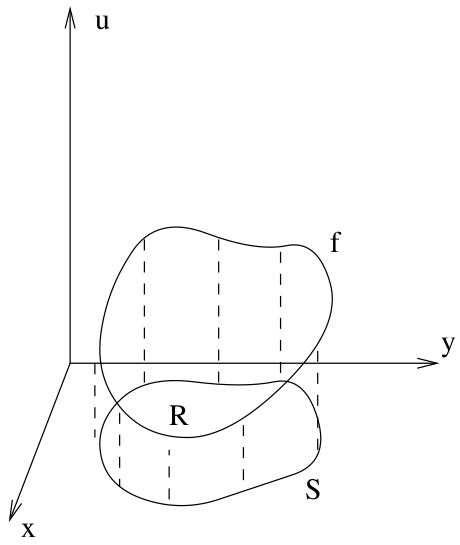
\includegraphics[width = \linewidth]{img/23/dirichlet}
    \column{0.45 \linewidth}
      \begin{itemize}
        \item graf $f(x,y)$ -- w 3D -- zamknięta krzywa
        \item graf $u(x,y)$ -- powierzchnia nad $R \bigcup S$, zawiera $f$
        \item $f$ -- brzeg
      \end{itemize}
  \end{columns}
\end{frame}

\begin{frame}
  Dowodzi się:
  \begin{itemize}
    \item istnienia i jednoznaczności rozwiązania zagadnienia Dirichleta
    \item $S$: prostokąt -- rozwiązanie -- szeregi Fouriera, \\
    okrąg, elipsa -- całka Poissona, szeregi Fouriera \\
    (i gdy można zastosować przekształcenia konforemne) \\
    ale: \textit{często rozwiązania analityczne -- wolnozbieżne}
    % Powyższe zdecydowanie powinno być zagnieżdżoną listą wypunktowaną, ale nie rozumiem struktury logicznej – czego dotyczy nawias?
  \end{itemize}

  W większości przypadków -- brak rozwiązań analitycznych (zamkniętych).
\end{frame}

\subsection*{Warunki graniczne dla r. Laplace'a -- zagadnienie Neumanna}
\subsubsection{Zagadnienie Neumanna}

\begin{frame}{Zagadnienie Neumanna}
  \begin{block}{Zagadnienie Neumanna}
    Wyznaczyć $u(x,y)$:
    \begin{itemize}
      \item ciągłą na $R \bigcup S$
      \item harmoniczną na $R$
      \item taką, że jej pochodna w kierunku normalnej wewnętrznej w~każdym punkcie $P$ brzegu $S$ przyjmuje zadane wartości:
      $$\frac{{\partial}u(x,y)}{{\partial}n} = g(x,y)$$
    \end{itemize}
  \end{block}
  Zagadnienie ma jednoznaczne rozwiązanie z dokładnością do stałego składnika.
\end{frame}

\subsection*{Warunki graniczne dla r. Laplace'a -- zagadnienie mieszane; Robina; trzeciego rodzaju}
\subsubsection{Zagadnienie mieszane; Robina; trzeciego rodzaju}

\begin{frame}{Zagadnienie mieszane; Robina; trzeciego rodzaju}
  \begin{block}{Zagadnienie mieszane; Robina; trzeciego rodzaju}
    $$\frac{{\partial}u}{{\partial}n} + H \cdot (u - h) = 0$$
    gdzie $H$,$h$ -- zadane funkcje
  \end{block}
  Powyższe zag. \textit{zag. brzegowe wewnętrzne} % Co za zag. zag.??? Mają być dwa??? (zagwarantuje, zagadnienie)??? A może należy zatytułować ten blok "zagadnienia brzegowe wewnętrzne" zamiast "zag. mieszane (...)"???
\end{frame}

\begin{frame}
  \begin{block}{Zagadnienia brzegowe zewnętrzne}
    Poszukiwana funkcja $u$ powinna być harmoniczną w obszarze nieograniczonym, położonym na zewnątrz powierzchni $S$.
  \end{block}
\end{frame}

\begin{frame}
  Podejście -- transformacja, inwersja
  \begin{columns}
    \column{0.45 \linewidth}
      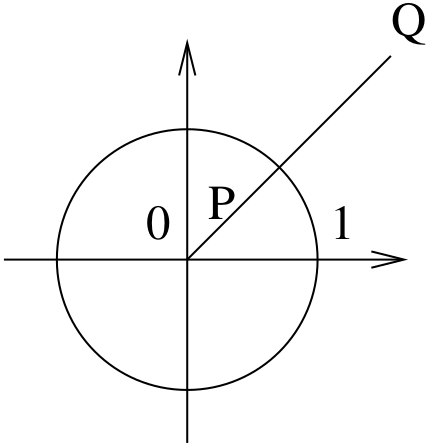
\includegraphics[width = \linewidth]{img/23/inwersja}
    \column{0.45 \linewidth}
      $$|0P| \cdot |0Q| = 1$$
  \end{columns}

  \vspace{5px}

  Zagadnienia brzegowe zewnętrzne mają jednoznaczne rozwiązania; brak ogólnej metody wyznaczania rozwiązań analitycznych.
\end{frame}


  \subsection{Przybliżenie równania Laplace'a układem równań różnicowych}

% Pierwszy link odnosi się do pliku na komputerze autora oryginalnego PDFa lub do lokalizacji na serwerze Bubaka, do której nie mamy dostępu (w co wątpię).
% Drugi link jest martwy, odpowiedni wydział odpowiedniej uczelni ma już nową stronę internetową, na której nie znalazłem podanych treści.

\begin{frame}{\large{Przybliżenie równania Laplace'a układem równań różnicowych}}
  \centerline{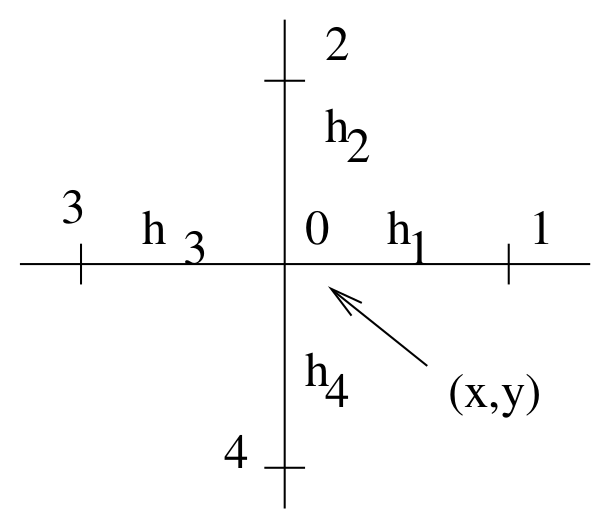
\includegraphics[width = 0.5 \linewidth]{img/23/przyblizanie}}
  $h>0, \qquad 0<h_i \le h, \qquad i = 1,2,3,4$ \\
  $u_i$  -- $u$ w punkcie $i$
\end{frame}

\begin{frame}
  Wyznaczamy parametry $\alpha_i$, $i=0, \dots ,4$ takie, by w $(x,y)$:
\begin{equation} \label{2}
\begin{split}
  u_{xx} + u_{yy} \equiv \alpha_0 \cdot u_0 + \alpha_1 \cdot u_1 + \alpha_2 \cdot u_2 + \alpha_3 \cdot u_3 + \alpha_4 \cdot u_4
\end{split}
\end{equation}

  Do $(\ref{2})$ podstawiamy rozwinięcia $u$ w szereg Taylora wokół $(x,y)$:
  $$ \begin{array}{l}
    u_1 = u_0 + u_x \cdot h_1 + \frac{1}{2} u_{x x} h_1^2 + O(h_1^3) \\
    u_2 = \ldots
  \end{array} $$

  Wtedy:
\begin{equation}
\begin{split}    
u_{x x} + u_{y y} \equiv u_0 \cdot (\alpha_0 + \alpha_1 + \alpha_2 + \alpha_3 + \alpha_4) + u_x \cdot (h_1 \alpha_1 - h_3 \alpha_3) + \\
    + u_y \cdot (\alpha_2 h_2 - \alpha_4 h_4) + \frac{1}{2} u_{x x} \cdot (h_1^2 \alpha_1 + h_3^2 \alpha_3) + \\
    + \frac{1}{2} u_{y y} \cdot (h_2^2 \alpha_2 + h_4^2 \alpha_4) + \sum_{i=1}^4 O(h_i^3)
\end{split}
\end{equation}
\end{frame}

\begin{frame}
  Porównując ze sobą odpowiednie współczynniki, a następnie rozwiązując układ pięciu równań, mamy:
  \begin{block}{}
    $$ \begin{array}{l}
    \alpha_0 = -2 \cdot \left[ \frac{1}{h_1 h_3} + \frac{1}{h_2 h_4} \right], \\
    \alpha_1 = \frac{2}{h_1 (h_1 + h_3)}, \\
    \alpha_2 = \frac{2}{h_2 (h_2 + h_3)}, \\ 
    \alpha_3 = \frac{2}{h_3 (h_1 + h_3)}, \\
    \alpha_4 = \frac{2}{h_4 (h_2 + h_4)}
    \end{array}$$
  \end{block}

  Zastąpienie równania Laplace'a przybliżeniem $(\ref{2})$ opiera się na:
  $$ \lim_{h \rightarrow 0} \sum_{i=1}^4 [O(h_i^3)] = 0$$ % W zasadzie w oryginale autor uparcie stosuje 0() zamiast O()...
\end{frame}

\begin{frame}
  Dla szczególnego, ważnego, przypadku:
  $$ h_1 = h_2 = h_3 = h_4 = h $$

  mamy:

  \begin{equation} \label{3} -4 u_0 + u_1 + u_2 + u_3 + u_4 = 0 \end{equation}

  z $(\ref{3})$ widać własność min-max:
  $$ u_0 = \frac{1}{4} (u_1 + u_2 + u_3 + u_4) $$

  czyli:
  \begin{block}{}
    $$ \min[u_1, u_2, u_3, u_4] \le u_0 \le \max[u_1, u_2, u_3, u_4] $$
  \end{block}

  Przedstawiony sposób transformacji PDE na równania różnicowe -- \textbf{uniwersalny}.
\end{frame}


  \subsection{Konstruowanie siatki}

\begin{frame}{Konstruowanie siatki}
  Dyskretyzacja zbioru punktów $R \bigcup S$
  $$ \left\{ \begin{array}{ll}
  (\overline{x}, \overline{y}) & \text{-- dowolny, ustalony punkt płaszczyzny} \\
  h > 0 & \text{-- rozmiar siatki (grid size)}
  \end{array} \right.$$
  \centerline{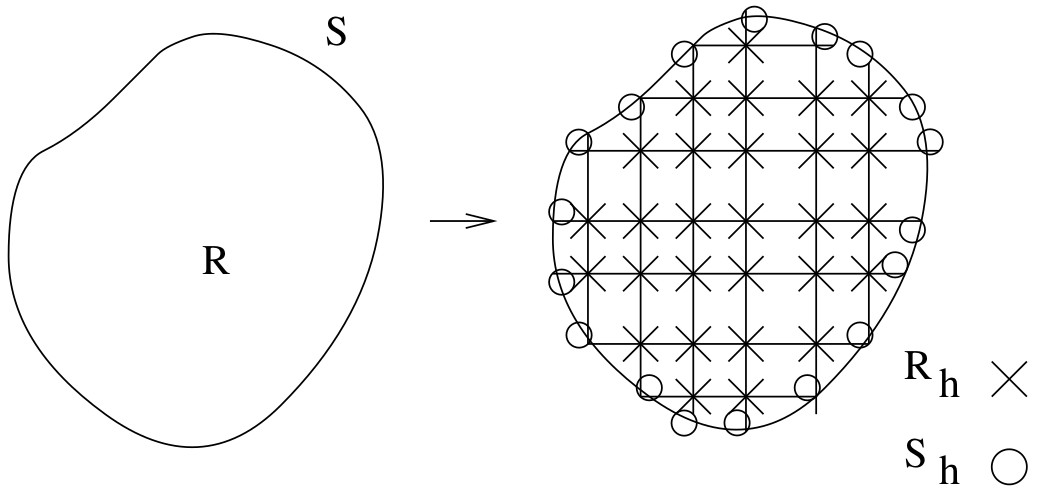
\includegraphics[width = \textwidth]{img/23/siatka}}
\end{frame}

\begin{frame}
  $$ \left\{ \begin{array}{ll}
  \text{zbiór punktów:} & \begin{array}{l} (\overline{x} + p \cdot h, \overline{y} + q \cdot h), \quad p,q = 0, \pm 1, \pm 2, \dots \\
    \rightarrow \text{zbiór punktów siatki płaskiej} \end{array}\\
  \text{zbiór linii:} & \left. \begin{array}{l}
    x = \overline{x} + p h \rightarrow \text{wertykalnych} \\
    y = \overline{y} + q h \rightarrow \text{horyzontalnych}
  \end{array} \right\} \begin{array}{l} \text{karta płaska} \\ \text{(planar lattice)} \end{array}
  \end{array} \right. $$
  $\rightarrow$ pokrywają całą płaszczyznę.
\end{frame}

\begin{frame}
  \begin{block}{}
    \begin{itemize}
      \item $R_h$ -- siatka wewnętrzna (interior grid): te punkty siatki, które należą do $R$
      \item $S_h^*$ -- punkty wspólne karty płaskiej i brzegu $S$
      \item $G_h^* = R_h \bigcup S_h^*$
      \item 4 sąsiedzi $(x,y) \in R_h \rightarrow$ 4 punkty $\in G_h^*$ najbliższe $(x,y)$ w 4 kierunkach
      \item $G_h$ -- podzbiór $G_h^*$ zawierający każdy punkt $R_h$ i 4 jego sąsiadów
      \item Brzeg siatki $S_h = G_h - R_h$
    \end{itemize}
  \end{block}
\end{frame}


  \subsection{Przykład}

\begin{frame}{Przykład}
  \centerline{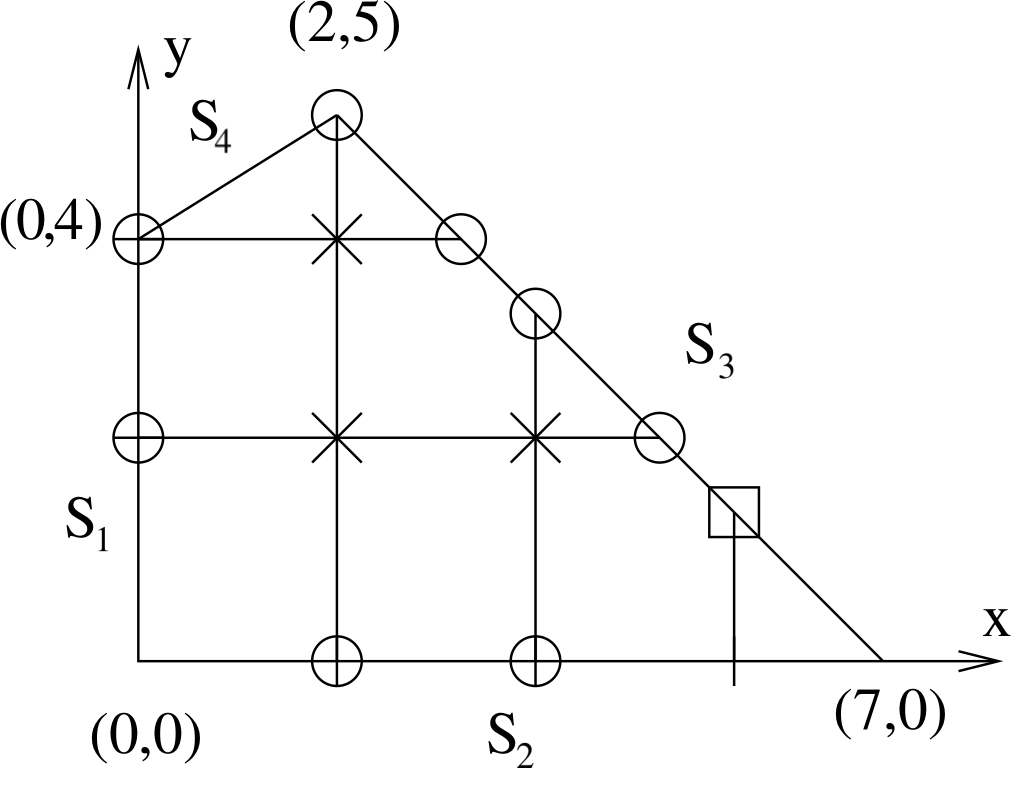
\includegraphics[height = 0.85 \textheight]{img/23/przyklad}}
\end{frame}

\begin{frame}
  \begin{block}{Oznaczenia}
    \begin{itemize}
      \item Czworokąt:
            $$(0,0), (7,0), (2,5), (0,4)$$
      \item $R$ -- wnętrze czworokąta
      \item $S$ -- brzeg czworokąta
      \item $S_i$, gdzie $i=1,\dots , 4$ -- boki czworokąta $\rightarrow$ brzeg $S$
    \end{itemize}
  \end{block}
\end{frame}

\begin{frame}
  Niech:
  \begin{itemize}
    \item $(\overline{x},\overline{y}) = (0,0);$
    \item $h=2$
  \end{itemize}

  Wówczas:
  \begin{itemize}
    \item Siatka wewnętrzna \begin{equation}R_h = \{(2,2),(2,4),(4,2)\} \end{equation}
    \item Punkty wspólne karty płaskiej i brzegu $S$: $S_h^* = S_i \bigcup S_2 \bigcup \text{(4 $\bigcirc$ i 1 $\square$ na $S_3$)}$ % CZY KWADRACIK TO POWINNA BYĆ *???
    \item Brzeg siatki:$$S_h = \{ (2,0),(4,0),(0,2),(5,2),(4,3),(3,4),(0,4),(2,5) \}\quad (\bigcirc)$$
  \end{itemize}
\end{frame}

\begin{frame}
  \begin{block}{Algorytm rozwiązywania zagadnienia Dirichleta}
    \begin{description}
      \item[krok 1]
        Dla ustalonych $h>0, (\overline{x},\overline{y})$
        \begin{itemize}
          \item tworzymy $R_h$ o $m$ punktach,
          \item tworzymy $S_h$ o $n$ punktach,
          \item numerujemy $R_h$ liczbami całkowitymi $[0,m]$ narastająco od lewej do prawej, z dołu do góry,
          \item numerujemy $S_h$ liczbami całkowitymi $[m+1, n+1]$ dowolnie.
        \end{itemize}
      \item[krok 2]
        W każdym $P_k(x,y) \in S_h$ podstawiamy $u_k = f(x,y)$.
    \end{description}
  \end{block}
\end{frame}

\begin{frame}
  \begin{block}{Algorytm rozwiązywania zagadnienia Dirichleta -- c.d.}
    \begin{description}
      \item[krok 3]
        W każdym $(x,y) \in R_h$ zapisujemy różnicowy odpowiednik równania Laplace'a:
        \begin{multline*}
          $$-2 \cdot ( \frac{1}{h_1 h_3} + \frac{1}{h_2 h_4}) \cdot u(x,y) + \\
          + \frac{2}{h_1 (h_1 + h_3)} u(x+h_1,y) + \frac{2}{h_2 (h_2 + h_4)} u(x,y + h_2) + \\
          + \frac{2}{h_3 (h_1 + h_s)} u(x-h_3,y)+\frac{2}{h_2 (h_2 + h_4)} u(x,y - h_4)=0$$ % 1. h_s W MIANOWNIOKU NIE MA ŻADNEGO SENSU (podejrzewam h_3)!!! 2. BARDZIEJ BYM SIĘ SPODZIEWAŁ h_4 PRZED NAWIASEM W MIANOWNIKU W OSTATNIM WYRAZIE
        \end{multline*}
        jeżeli zaś punktem sąsiednim $(x,y)$ jest punkt $\in S_{h^-}$ % CZYŻBY CHODZIŁO O S_h^* ???
        to $u$ w punkcie sąsiednim zastępujemy przez wartość $f(x,y) \rightarrow$ krok 2.

        Otrzymujemy układ $m$ równań o $m$ niewiadomych.
      \item[krok 4]
        Rozwiązanie układu równań.
    \end{description}
  \end{block}
\end{frame}

\begin{frame}
  \begin{block}{Algorytm rozwiązywania zagadnienia Dirichleta -- c.d.}
    \begin{description}
      \item[krok 5]
        Dyskretna funkcja $u_i$, gdzie $i=1,2, \dots ,m+n$, określona tylko na $R_h + S_h$, reprezentuje przybliżone rozwiązanie zagadnienia Dirichleta.
    \end{description}
  \end{block}

  \begin{block}{Stosowanie powyższego algorytmu opiera się na poniższych faktach}
    \begin{enumerate}
      \item przybliżone rozwiązanie zagadnienia Dirichleta istnieje i jest jednoznaczne,
      \item dla szerokiej klasy zagadnień rozwiązanie numeryczne jest zbieżne do analitycznego z $h \rightarrow 0$,
      \item otrzymany układ równań może być rozwiązany metodą SOR dla dowolnego przybliżenia początkowego z $ \omega \in (0,2)$; dla pewnych klas zagadnień można znaleźć optymalne wartości $\omega$ (najszybsza zbieżność procesu iteracyjnego).
    \end{enumerate}
  \end{block}
\end{frame}

\begin{frame}
  \begin{exampleblock}{Przykład}
    $S$: 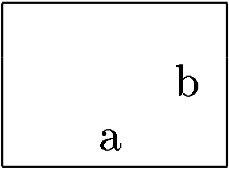
\includegraphics[width = 0.2 \textwidth]{img/23/prostokat}
    $$ \omega = \frac{2}{1 + \sqrt{1 - \lambda ^2}}, \quad \lambda = \frac{1}{2} \left( \cos \frac{\pi \cdot h}{a} + \cos \frac{\pi \cdot h}{b} \right)$$
  \end{exampleblock}

  \begin{alertblock}{Uwaga}
    Układ równań liniowych ma macierz diagonalnie dominującą $\Rightarrow$ wynik uporządkowania, określonego w kroku 3: na diagonali -- współczynniki przy $u(x,y)$.
  \end{alertblock}
\end{frame}

\begin{frame}
  \textit{Powrót do przykładu}

  \begin{itemize}
    \item $R$ -- wnętrze czworoboku
    \item $S$ -- bok czworoboku
    \item zagadnienie Dirichleta $z$
    \item $f(x,y) = x^2 - y^2$ na $S$
    \item $(\overline{x}, \overline{y}) = (0,0), h=2$
    \item $R_h$: $1,2,3$
    \item $S_h$: $4,5, \dots , 11$
  \end{itemize}
\end{frame}

\begin{frame}
  \centerline{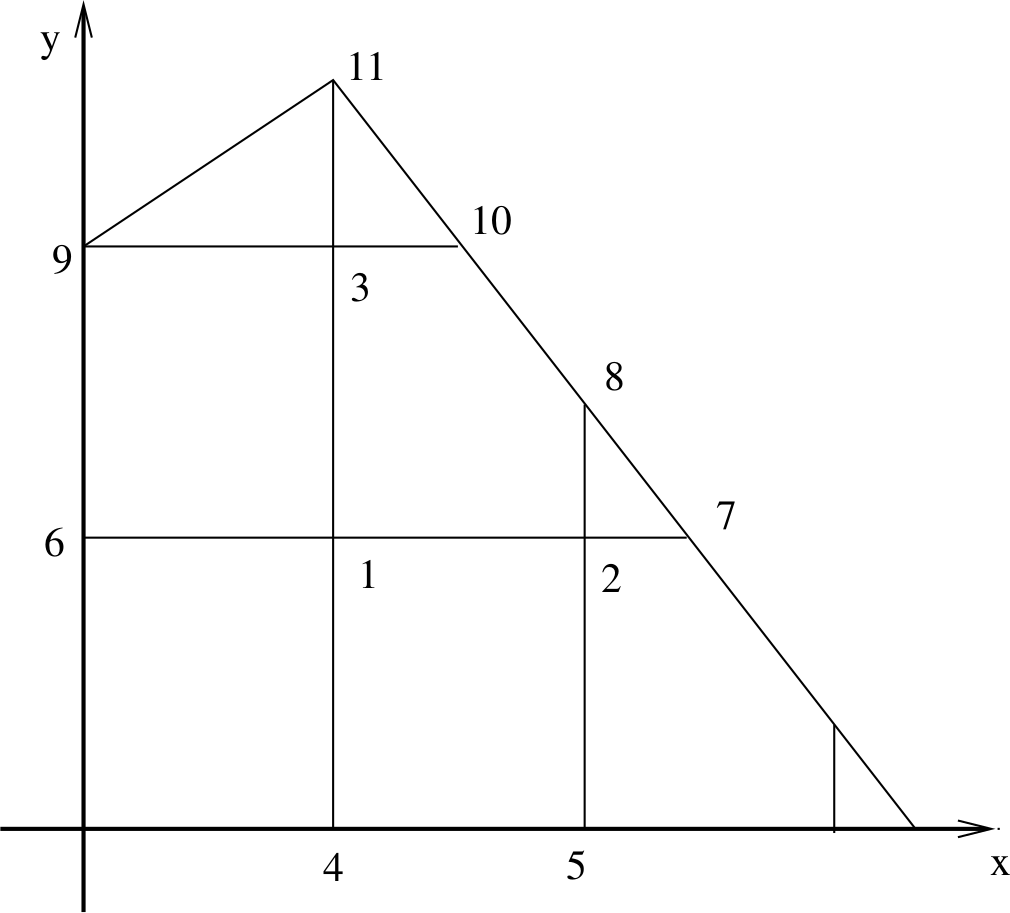
\includegraphics[height = 0.85 \textheight]{img/23/przyklad2}}
\end{frame}

\begin{frame}
  $$ u_4 = 4, u_5 = 16, u_6 = -4, u_7 = 21 $$
  $$ u_8 = 7, u_9 = -16, u_{10} = -7, u_{11} = -21 $$

  \begin{multline*}
    $$ -2 (\frac{1}{h_1 h_3} + \frac{1}{h_2 h_4}) u_0 + \\
    + \frac{2 u_1}{h_1 (h_1 + h_3)} + \frac{2 u_2}{h_2 (h_2 + h_4)} + \frac{2 u_3}{h_3 (h_1 + h_3)} + \frac{2 u_4}{h_4 (h_2 + h_4)} = 0 $$
  \end{multline*}
\end{frame}

\begin{frame}
    $$ \left\{ \begin{array}{ll}
    -u_1 + \frac{1}{4} u_2 + \frac{1}{4} u_3 + \frac{1}{4} (-4) + \frac{1}{4} \cdot 4 & =0 \\
    -2 u_2 + \frac{2}{3} \cdot 21 + \frac{2}{3} \cdot 7 + \frac{1}{3} u_1 + \frac{1}{3} \cdot 16 & =0 \\
    -2 u_3 + \frac{2}{3} (-7) + \frac{2}{3} (-21) + \frac{1}{3} (-16) + \frac{1}{3} u_1 & =0
    \end{array} \right. $$

  $$ \left\{ \begin{array}{llll}
  - u_1 & + \frac{1}{4} u_2 & +\frac{1}{4} u_3 & =0 \\
  \frac{1}{3} u_1 & -2 u_2 && =-24 \\
  \frac{1}{3} u_1 && -2 u_3 & =24
  \end{array} \right. $$

  Rozwiązanie: $u^T = (0, 12, -12)$.
\end{frame}


  \section{Równania paraboliczne}

\begin{frame}{Równania paraboliczne -- wstęp}
  \begin{block}{Prototyp: równanie transportu ciepła}
    \begin{equation}\label{7} u_{x x} = u_t \end{equation}
  \end{block}
\end{frame}


  \subsection{Initial value problem}

\begin{frame}{Initial value problem}
  \begin{description}
    \item[Dane:]
      $f(x)$ ciągła dla wszystkich $x$
    \item[Szukana:]
      $u(x,t)$
      \begin{itemize}
        \item określona i ciągła \\ dla $-\infty < x < \infty, t \ge 0$
        \item spełniająca $(\ref{7})$ \\ dla $-\infty < x < \infty, t > 0$
        \item spełniająca $u(x,0) = f(x)$ \\ dla $-\infty < x < \infty, t = 0$
      \end{itemize}
  \end{description}
\end{frame}

\begin{frame}
  \centerline{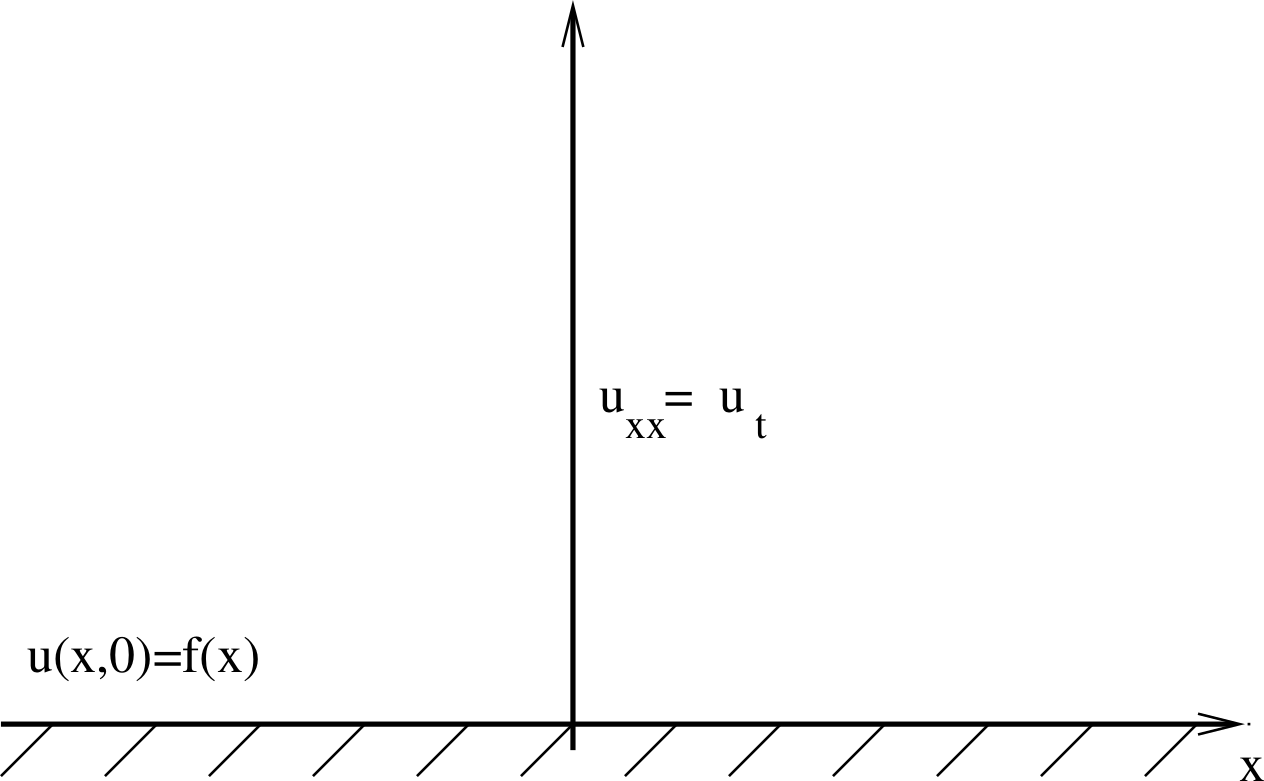
\includegraphics[height = 0.85 \textheight]{img/23/ivp}}
  (half-plane)
\end{frame}

\begin{frame}
  Rozwiązanie $\rightarrow$ całka Fouriera
  \begin{alertblock}{Problem}
    \begin{itemize}
      \item przypadek nieliniowy $\rightarrow$ ?
      \item kłopoty z wyznaczeniem wartości w $(x,t)$
    \end{itemize}
  \end{alertblock}
\end{frame}


  \subsection{Initial boundary problem}

\begin{frame}{Initial boundary problem}
  \begin{description}
    \item[Dane:]
      \begin{itemize}
        \item stała $a>0$
        \item trzy ciągłe funkcje: $g_1(t)$, $g_2(t)$, $f(x)$ dla $ \left\{ \begin{array}{l} t \ge 0 \\ 0 \le x \le a \end{array} \right. $
      \end{itemize}
    \item[Szukana:]
      $u(x,t)$:
      \begin{itemize}
        \item określona i ciągła \\ dla $0 \le x \le a, t \ge 0$,
        \item spełniająca $(\ref{7})$ \\ dla $0 < x < a, t > 0$,
        \item spełniająca:
        $$ \left\{ \begin{array}{lrl}
        u(x,0) = f(x), & 0 \le x \le a & \text{initial condition} \\
        u(0,t) = g_1(t), & t \ge 0 & \text{boundary condition} \\
        u(a,t) = g_2(t), & t \ge 0 & \text{boundary condition}
        \end{array} \right. $$
      \end{itemize}
  \end{description}
\end{frame}

\begin{frame}
  \centerline{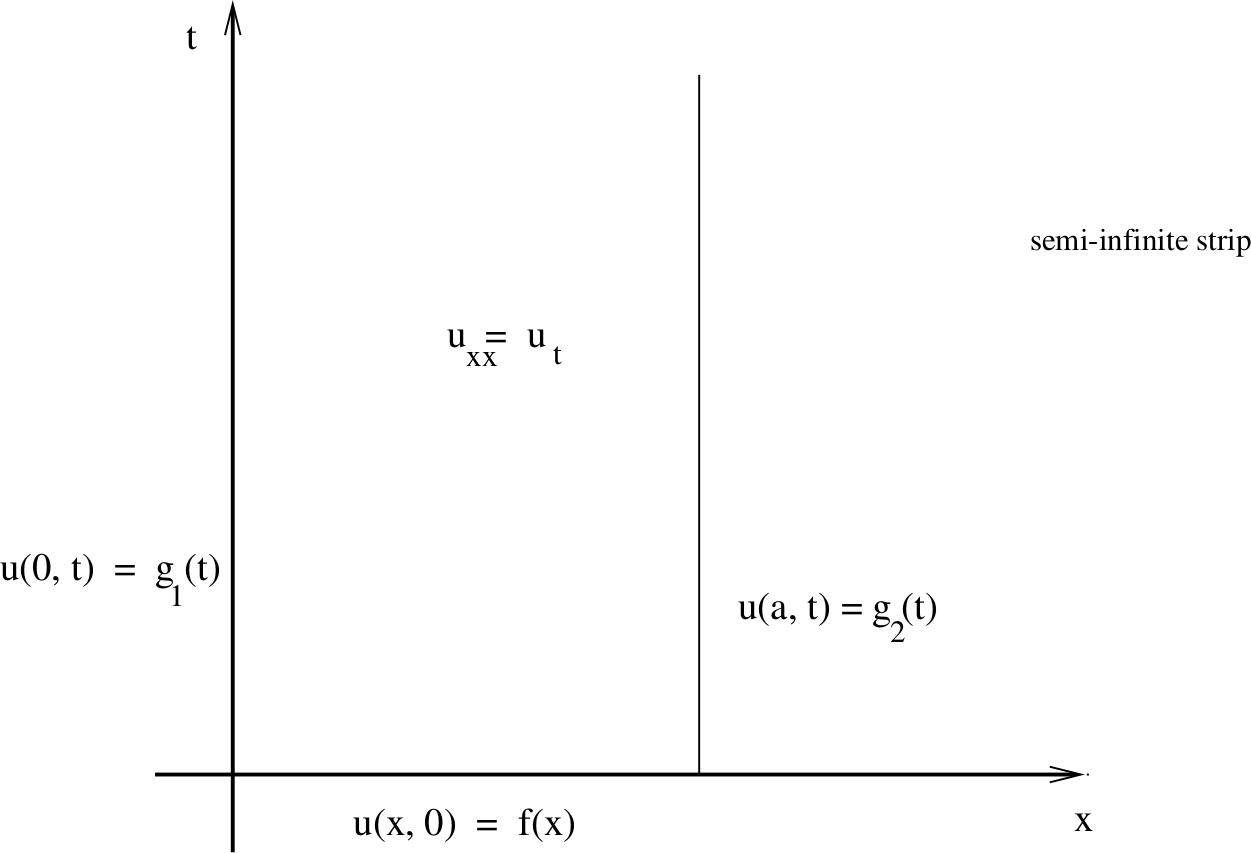
\includegraphics[height = 0.85 \textheight]{img/23/ibp}}
\end{frame}

\begin{frame}
  Rozwiązanie $\rightarrow$ szeregi Fouriera

  \begin{alertblock}{Problem}
    Ten sam problem jak poprzednio...
  \end{alertblock}
\end{frame}


  
\subsection{Stabilność}
\begin{frame}{Stabilność}
  \begin{block}{Powód:}
\begin{itemize}
    \item $ 0  \le t \leq \alpha $
    \item $\text{wybór } \Delta t $
\end{itemize}
  \end{block}
    
      $\Delta x = h $ \\
      $\Delta t = k$ \\
      $ R = \{P(x,t): 0 < x < a, t > 0\}$ \\
      $S - \text{brzeg R}$ \\
      $R_h = x \rightarrow \text{punkty wewnętrzne}$ \\
      $S_h = 0 \rightarrow \text{punkty brzegowe}$
  \end{frame}

\begin{frame}
  \centerline{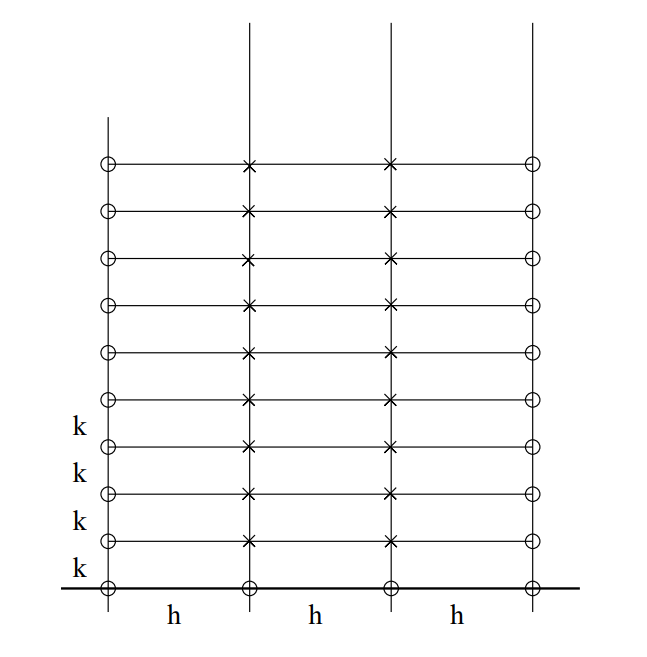
\includegraphics[height = 0.85 \textheight]{img/23/stabilnosc}}
\end{frame}

\begin{frame}
$ m^{th} \text{ row of grid points:}$
$$y = m \cdot k$$
\centerline{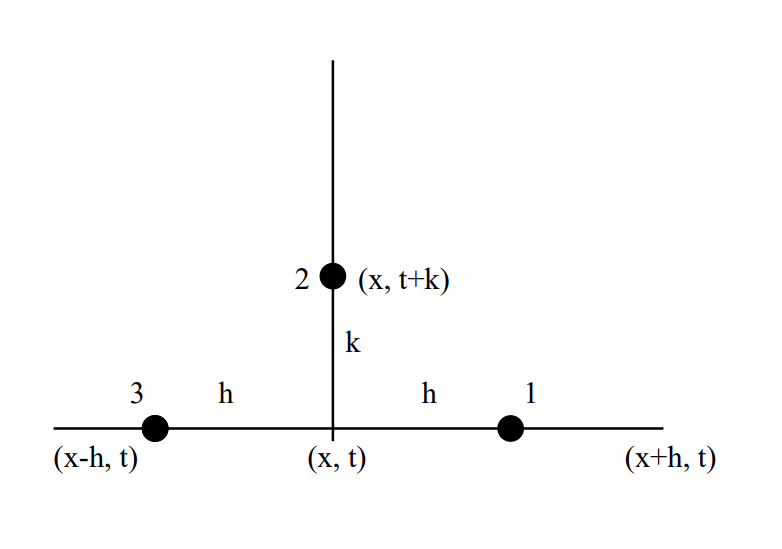
\includegraphics[height = 0.55 \textheight]{img/23/stabilnosc2}}

\begin{block}{}
   $$ \begin{array}{l}
   u_{xx}(x,t) = \frac{u(x-h,t)-2 \cdot u(x,t) + u(x+h,t)}{h^{2}}, \\ \\
   u_t (x,t)= \frac{u(x,t+k)-u(x,t)}{k}
   \end{array}$$
 \end{block}

\end{frame}

\begin{frame}
Po podstawieniu do (\ref{7}) ($u_{x x} = u_t$) i uporządkowaniu:
$$u(x,t+k) = u(x,t) + \frac{k}{h^2}[u(x+h,t)-2\cdot u(x,t)+u(x-h,t)]$$
wprowadzając: $\lambda = \frac{k}{h^2}$, uzyskujemy:
$$u(x,t+k) = \lambda \cdot u(x+h,t)+(1-2\lambda)u(x,t)+\lambda \cdot u(x-h,t)$$
używając oznaczeń z rysunku:
$$u_2 = \lambda \cdot u_1+(1-2\lambda)\cdot u_0+\lambda \cdot u_3$$


$$ \textcolor{blue}{\text{Algorytm (Explicit Method):}}\left
\{ \begin{array}{lrl}
       \text{konstrukcja siatki}\\
       \text{wiersz po wierszu} \rightarrow \text{kolejno w górę.}
        \end{array} \right. $$
\end{frame}

\begin{frame}
Rozwiązania $\rightarrow$ mają własność min-max (physically reasonable)
\center{stable if any only if is physically reasonable}
\centerline{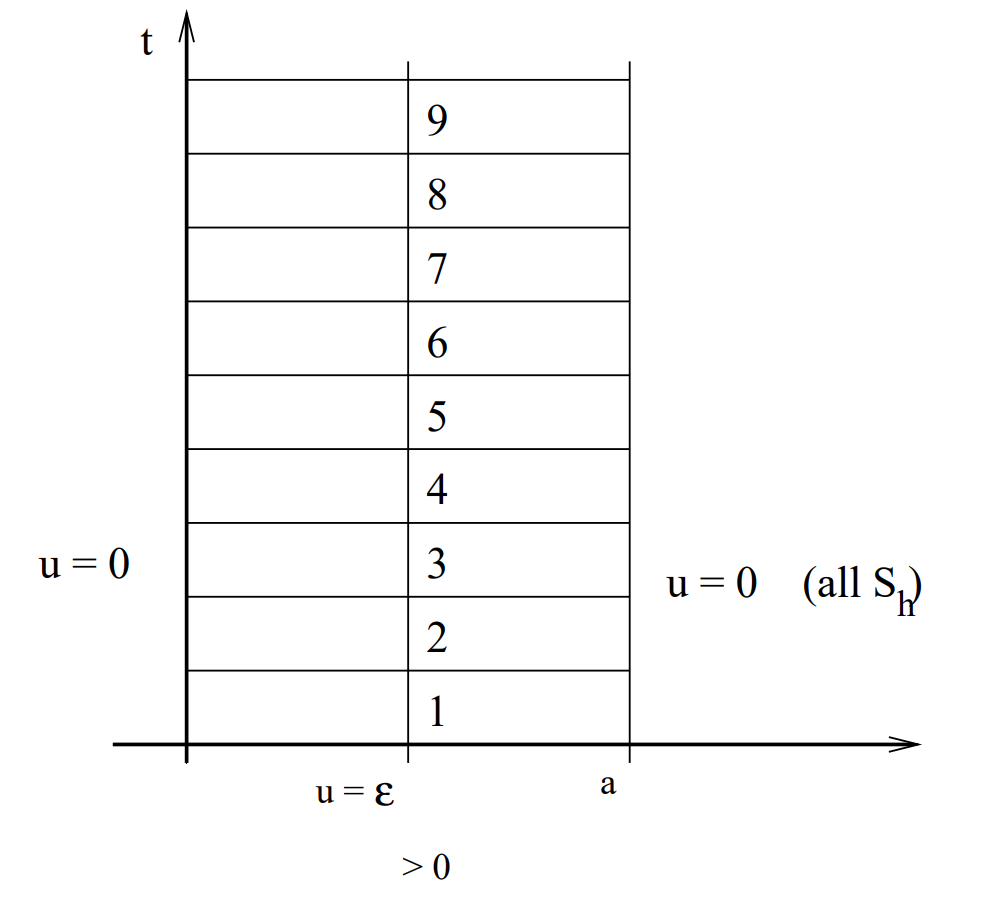
\includegraphics[height = 0.70 \textheight]{img/23/stabilnosc4}}
\end{frame}

\begin{frame}
$\Delta x = \frac{a}{2} , \quad \Delta t = k$ \\
\vspace{5mm}
$u_1 = (1 - 2 \lambda)\varepsilon ,    u_2 = (1 - 2\lambda )^2\varepsilon , u_3 = (1-2\lambda)^3 \cdot \varepsilon , ... u_m = (1-2\lambda)^m\cdot \varepsilon$ \\
\vspace{5mm}
$\ 0 \leq u \leq \varepsilon  \quad \text{na} \ S_n$
$$0 \leq (1-2 \lambda)^m \cdot \varepsilon \leq \varepsilon$$
$\Longrightarrow 0 \leq \lambda \leq \frac{1}{2}$
\end{frame}

  
\subsection{Explicit Method}
\begin{frame}{Explicit Method}

\begin{block}{}
\begin{flushleft}
    \begin{enumerate}
      \item [1.]  
   $\text{Ustalić } \Delta x = h , \ \Delta t = k \text{ tak, aby} \quad \lambda = \frac{k}{h^2} \leq \frac{1}{2} . $\\ $\text{Skonstruować } R_h \text{ i } S_h $
      
      \item [2.] W oparciu o: \begin{itemize}
\item warunek początkowy i brzegowy
\item wzór $u(x, t+k) = \lambda \cdot u(x+h, t) + (1 - 2\lambda) u (x,t) + \lambda u(x-h, t)$ \\
\textcolor{blue}{wyznaczyć $u$ we wszystkich punktach pierwszego wiersza $R_h$}
\end{itemize} 
	\item [3.] W oparciu o:
\begin{itemize}
\item warunek brzegowy
\item wartość $u$ w wierszu $k, k \geq 1, $ \\
\textcolor{blue}{wyznaczyć $u$ w wierszu $k+1$, $k$ = 1,2,...}
\end{itemize}
    \end{enumerate}
\end{flushleft}
  \end{block}

 
\end{frame}


  
\subsection{Implicit Method}
\begin{frame}{Implicit Method}

\begin{block}{}
   $$ \begin{array}{l}
   \text{Dla } t = 100, h = \frac{1}{100} \\
   \end{array}$$
 \end{block}
 
z $\lambda \leq \frac{1}{2} \Rightarrow \Delta t = k \leq \frac{1}{2}(\frac{1}{100})^2 = 5 \cdot 10^{-5}$  \\
  \begin{alertblock}{Problem}
    Dla znalezienia rozwiązania dla $t = 100$ potrzeba $2 \cdot 10^6$ wierszy!
  \end{alertblock}
Rozwiązaniem jest zmiania podstawowego równania: 
       \centerline{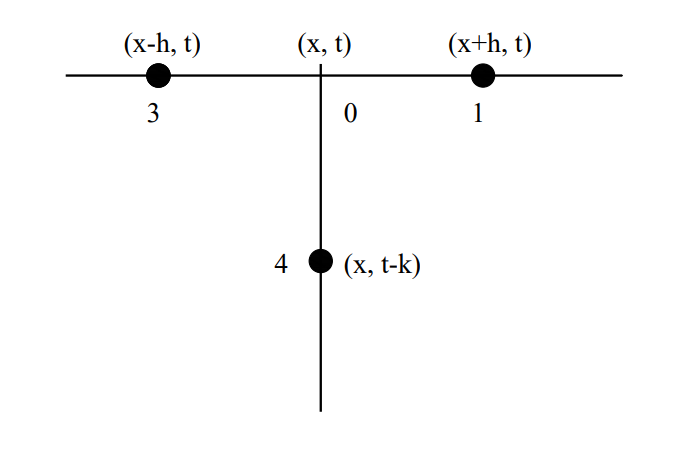
\includegraphics[width = 0.5 \linewidth]{img/23/implicit}}
\end{frame}

\begin{frame}
\begin{equation}\frac{u(x-h,t) - 2 \cdot u(x,t) + u(x+h, t)}{h^2} = \frac{u(x,t) - u(x,t - k)}{k}\end{equation}
co możemy zapisać: \begin{equation}\lambda \cdot u(x-h,t) - (1+2 \cdot \lambda)u(x,t) + \lambda \cdot u(x+h,t) = -u(x,t-k)\end{equation} 
albo:\begin{equation}\lambda \cdot u_3 - (1+2\cdot \lambda) \cdot u_0 + \lambda \cdot u_1 = - u_4 \rightarrow \text{stabilny dla wszystkich } \lambda\end{equation}

\begin{block}{}
Tym razem do wyznaczenia rozwiązań dla każdego wiersza trzeba
rozwiązać układ równań liniowych z macierzą trójdiagonalną, diagonalnie dominującą.
\end{block}

\end{frame}

  
\subsection{The Crank--Nicolson Method}
\begin{frame}{The Crank-Nicolson Method}

\begin{block}{}
   \center{symmetry in the construction of difference equations \\ $\rightarrow$
better accurancy} 
 \end{block}
 
\begin{equation}\underline{\frac{\partial u}{\partial t} \Big \vert _{A}\cong \frac{u(x,t) - u(x,t - h)}{k}}\end{equation} w oparciu o punkty symetryczne wzgl. A
 
 \centerline{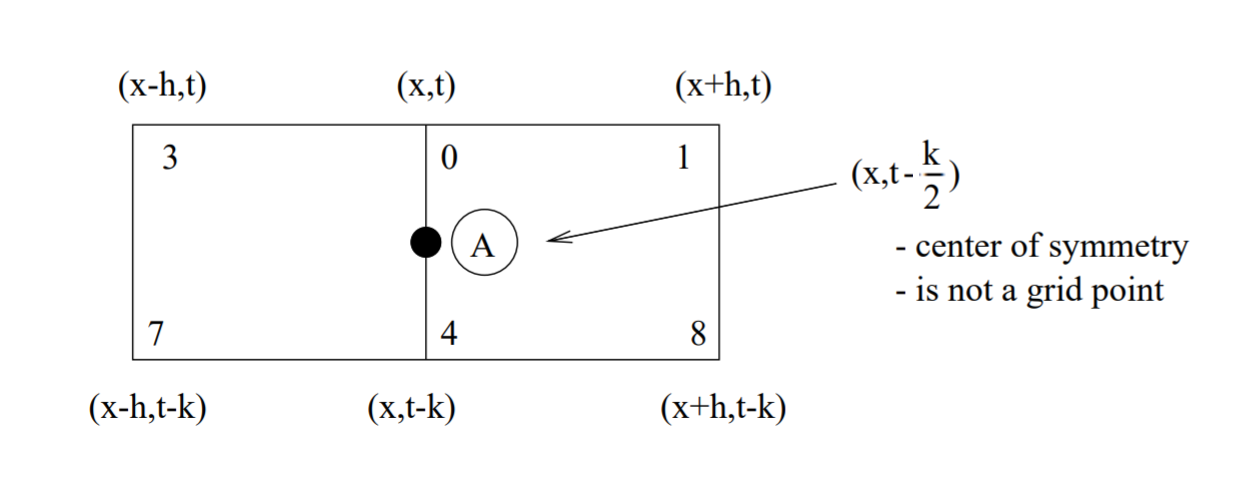
\includegraphics[width = 1 \linewidth]{img/23/crank}}
\end{frame}

\begin{frame}
\begin{equation} \frac{\partial ^2 u}{\partial x^2} \Big \vert _{4}\approx \frac{u(x - h,t - k) - 2 \cdot u(x,t - k) + u(x + h, t - k)}{h^2}\end{equation}
\begin{equation} \frac{\partial ^2 u}{\partial x^2} \Big \vert _{0}\approx \frac{u(x - h,t) - 2 \cdot u(x,t) + u(x + h, t)}{h^2} \end{equation}
to:
\begin{equation} \frac{\partial ^2 u}{\partial x^2} \big \vert _{A} = \frac{1}{2} \cdot \left ( \frac{\partial ^2 u}{\partial x^2} \Big \vert _{0} + \frac{\partial ^2 u}{\partial x^2} \Big \vert _{4} \right )\end{equation}
\textbf{W met. ,,Implicit'' wprowadzamy:}
\begin{multline} \lambda \cdot u(x-h,t) - (1+2 \cdot \lambda)\cdot u(x,t) + \lambda \cdot (x+h,t) = \\
 -\lambda \cdot u(x-h,t-k) - (1-2 \cdot \lambda) \cdot u(x,t-k) - \lambda \cdot u(x+h,t-k)\end{multline}
czyli:
$$ \underline{\lambda \cdot u_3 - (1+2 \cdot \lambda) u_0 + \lambda u_1 = -\lambda \cdot u_7 - (1-2 \cdot \lambda) u_4 - \lambda u_8}$$
\end{frame}

  \section{Równanie falowe}

\begin{frame}{Równanie falowe}
  \begin{block}{2 sposoby:}
\begin{itemize}    
\item równanie różniczkowe cząstkowe 2-go rzędu
\item równoważny układ 2 równań 1-go rzędu
\end{itemize}
  \end{block}
\begin{equation} \label{etykieta}\underline{u_{xx} - u_{tt} = 0} \end{equation}
\end{frame}



  \subsection{The Cauchy problem = initial value problem}
\begin{frame}{The Cauchy problem = initial value problem}

  \begin{block}{Definition on a half-plane}
  Szukamy u(x,t):
\begin{itemize}    
\item określonej
\item ciągłej
\end{itemize}
	 dla:
   
$-\infty < x < \infty, t \ge 0 $ \\
spełniającej (\ref{etykieta}) dla \\
$-\infty < x <\infty, t > 0 $


oraz spełniającej warunki początkowe:
\begin{equation}u(x,0) = f_1(x), -\infty < x < \infty\end{equation}
\begin{equation}u_t(x,0) = f_2(x), -\infty < x < \infty\end{equation}
$f_1(x), f_2(x) $ -- zadane funkcje
\end{block}
\end{frame}

\begin{frame}
  \centerline{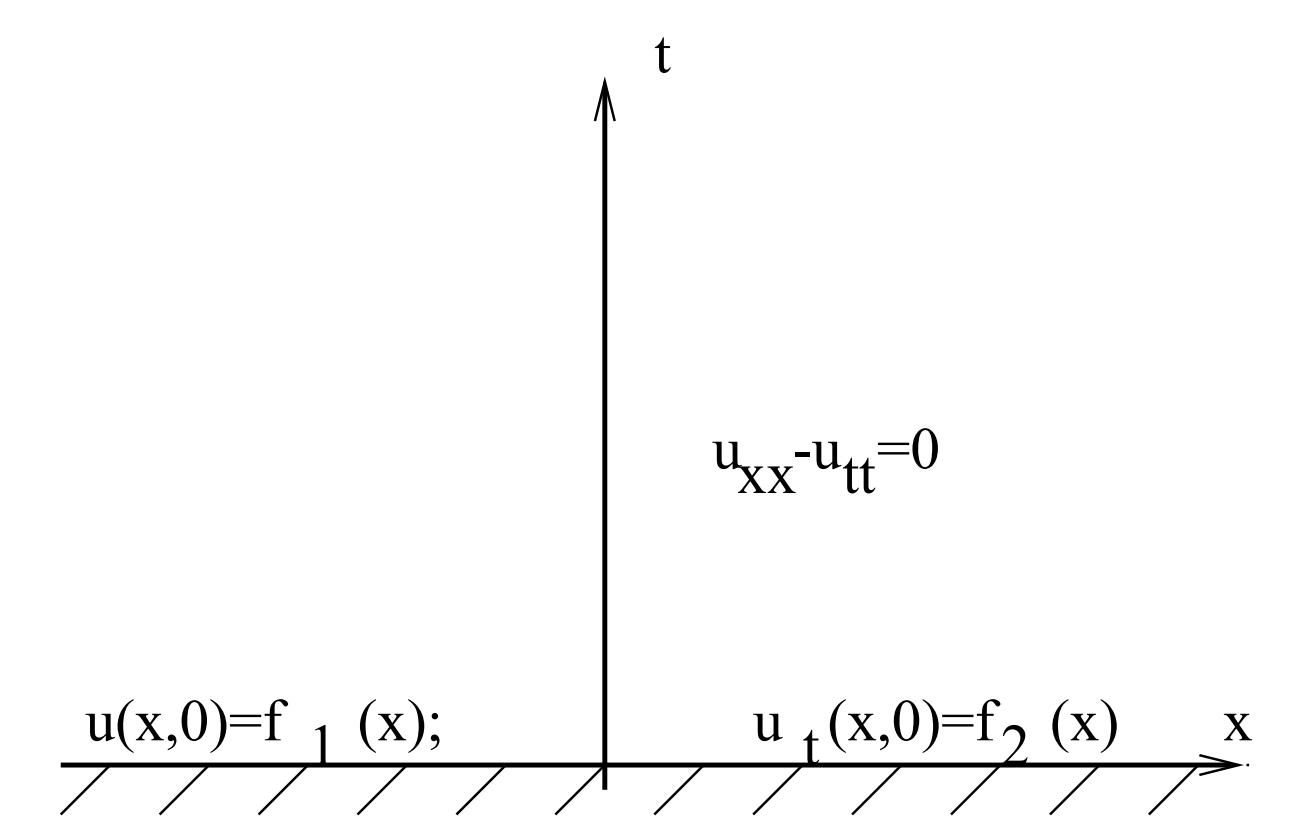
\includegraphics[height = 0.85 \textheight]{img/23/cauchy}}
\end{frame}

  


\subsection{Initial boundary problem}

\begin{frame}{An initial boundary problem}

 \begin{block}{Definition on a semi-infinite strip}
Dane:
\begin{itemize}    
\item $a>0$
\item $g_1(t), g_2(t); t \ge 0$
\item $f_1(x), 0 \le x\le a$
\item $f_2(x), 0 < x < a$
\end{itemize}
	
\end{block}

\end{frame}

\begin{frame}
  \centerline{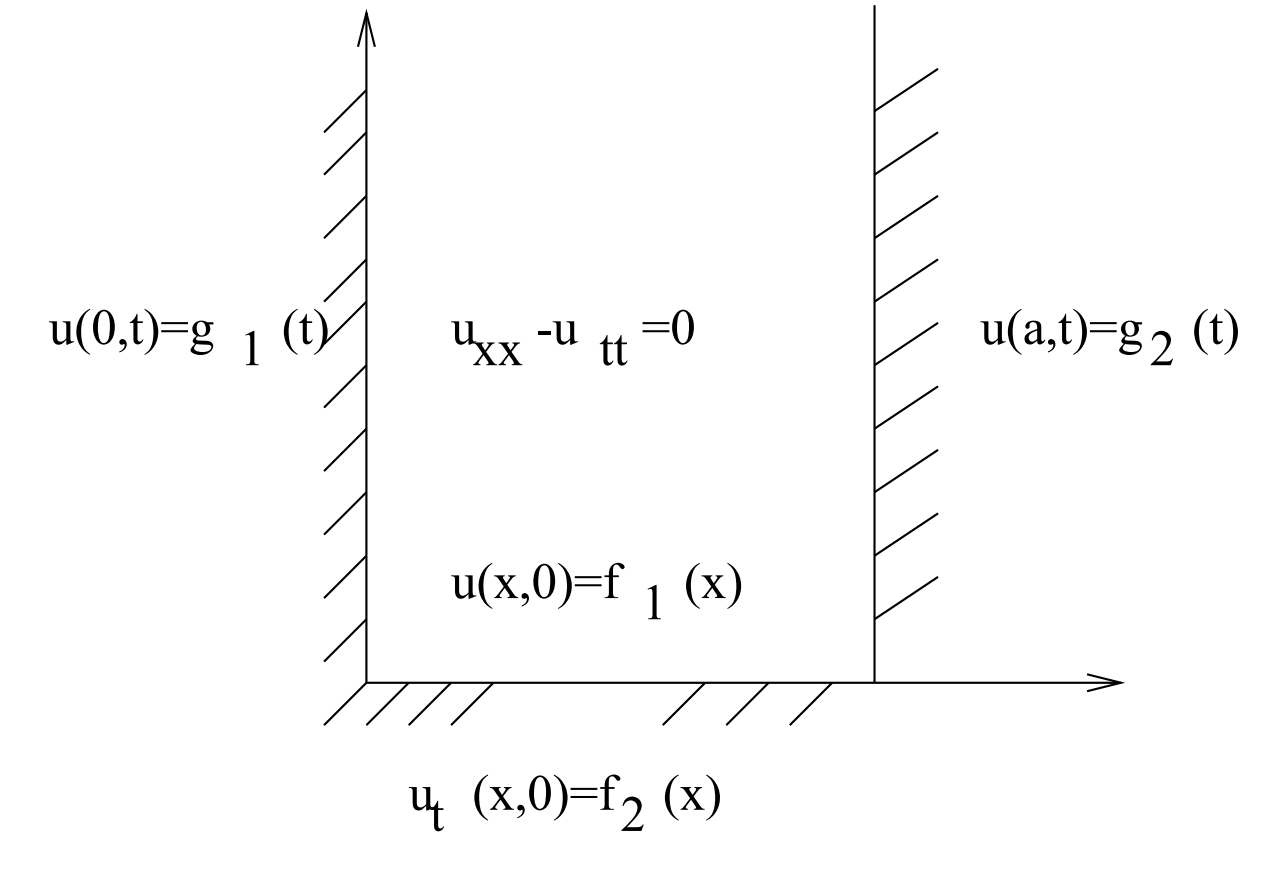
\includegraphics[height = 0.85 \textheight]{img/23/initial_boundary}}
\end{frame}

\begin{frame}
  Szukana funkcja u(x,t), ciągła dla $0 < x < a, t > 0$
spełnia warunek początkowy i brzegowy:

\begin{subnumcases}{\text{initial condition}}
 u(x,0) = f_1(x), 0 \le x \le a \label{first} \\
 u_t(x,0) = f_2(x), 0 < x < a \label{second}
\end{subnumcases}

\begin{subnumcases}{\text{boundary condition}}
 u(0,t) = g_1(t), t\ge 0  \\
u(a,t) = g_2(t), t \ge 0
\end{subnumcases}


  \begin{block}{Rozwiązania}
Cauchy-problem $\to$ wzór D'Alemberta \\
initial boundary problem $\to$ szereg Fouriera
 
  \end{block}
\begin{alertblock}{Ale...}
\begin{itemize}
\item nie gdy nieliniowe
\item trudności z wyznaczeniem
\end{itemize}
\end{alertblock}
\end{frame}


  
\subsection{Stabilność}
\begin{frame}{Stabilność}
$\to$ initial boundary problem

  \begin{block}{}
$0 \le x \le a \text{ podział na } n \to \Delta x = \frac{a}{h} = h$
$R: \{ (x,y): 0 < x< a, t > 0\}$
  \end{block}
$S$ - brzeg $R$
$\Rightarrow \text{tworzymy } R_h, S_h$


 \rightline{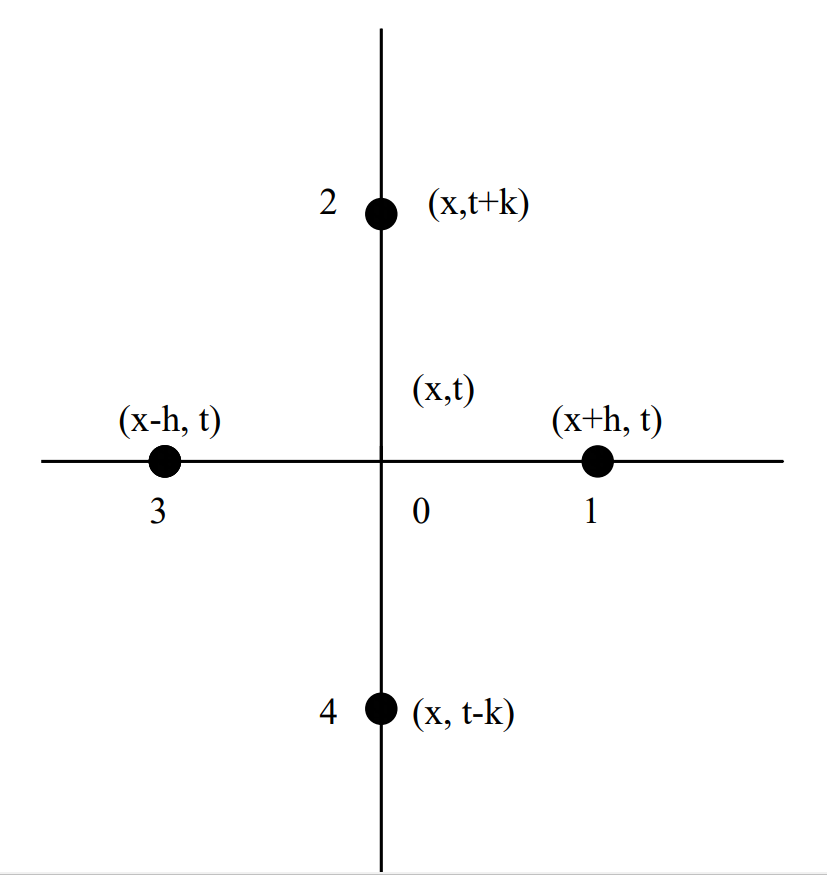
\includegraphics[height = 0.62 \textheight]{img/23/stab1}}
\end{frame}

\begin{frame}
$$u_{xx} = \frac{u(x-h,t)-2u(x,t)+u(x+h,t)}{h^2},$$
$$u_{tt} = \frac{u(x,t+k)-2u(x,t)+u(x,t-k)}{k^2},$$
czyli przybliżeniem (\ref{etykieta}) jest: \\
\begin{equation} \label{21} u(x,t+k) = 2\cdot u(x,t) - u(x,t-k) + \frac{k^2}{h^2}[u(x-h,t)-2u(x,t)+u(x+h,t)] \end{equation}
Dla wyznaczenia $u$ w pierwszym wierszu $\Rightarrow$ przybliżenie (\ref{second}):
$$u_t(x,0) \approx \frac{u(x,k) - u(x,0)}{k} = f_2(x)$$
czyli:
\begin{equation} \label{22} u(x,k) = u(x,0) + k \cdot f_2(x) \end{equation}
\end{frame}

\begin{frame}
  \begin{exampleblock}{Przykład}
      \begin{enumerate}[I.]
       \item $u(x,0) = x \quad 0 \ge x \ge 1$ \\
	\item $u_t(x,0) = 1\quad 0 < x < 1$ \\
      \item $u(0,t) = 0 \quad t \le 0$ \\
	\item $u(1,t) = 1 \quad t \le 0$
\end{enumerate}
  \end{exampleblock}
\vspace{5mm}
Zobaczymy, co będzie, gdy h = $\frac{1}{6}, k =\frac{1}{2}$ i pominiemy w. b. III) i IV) \\
\vspace{5mm}
z (\ref{22}) i I): $u_1 = \frac{2}{3}, u_2 = \frac{5}{6}, u_3 = 1, u_4 = \frac{7}{6}, u_5 = \frac{4}{3}$ \\
\vspace{3mm}
z (\ref{21}): $u_7 = \frac{4}{3}, u_8 = \frac{3}{2}, u_9 = \frac{5}{3}$
\end{frame}

\begin{frame}
 \centerline{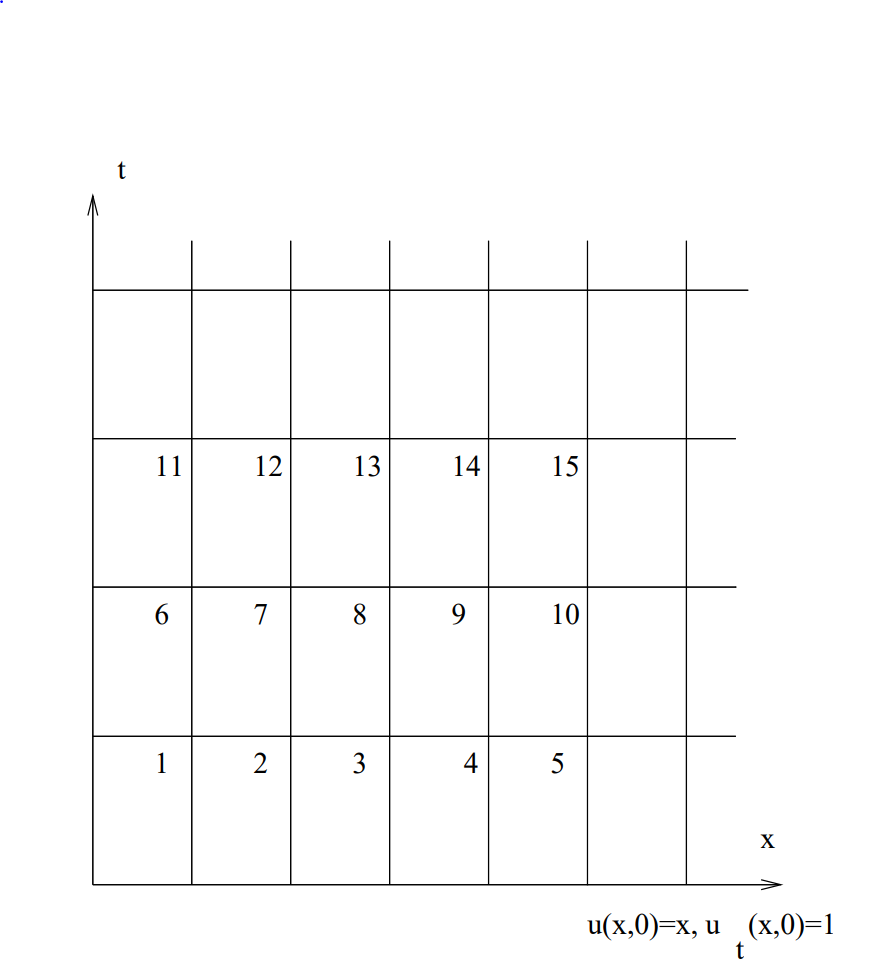
\includegraphics[height = 1 \textheight]{img/23/stab2}}
\end{frame}

\begin{frame}
\begin{alertblock}{Ale...}
\begin{itemize}
  \item  $u_6, u_{10} $ -- nie może być wyznaczone! 	
\item i wreszcie $u_{13} = 2$
 \item przy pominiętych III) i IV) \\
$\Rightarrow u$ tylko w trójkącie $(0,0), (1,0),\underbrace{\left ( \frac{1}{2}, \frac{1}{2} \right )}_{\#3} ! $
\end{itemize}
 \end{alertblock}

\vspace{6mm}
usunięcie niezgodności: $k \le h$ (warunek stabilności dla (\ref{21})) \\
$\Rightarrow$ jest to \textbf{Explicit Method for Initial-Boundary Problems}
\end{frame}




  \subsection{Implicit Methods for Initial-Boundary Problems}

\begin{frame}{Implicit Methods for Initial-Boundary Problems}

\rightline{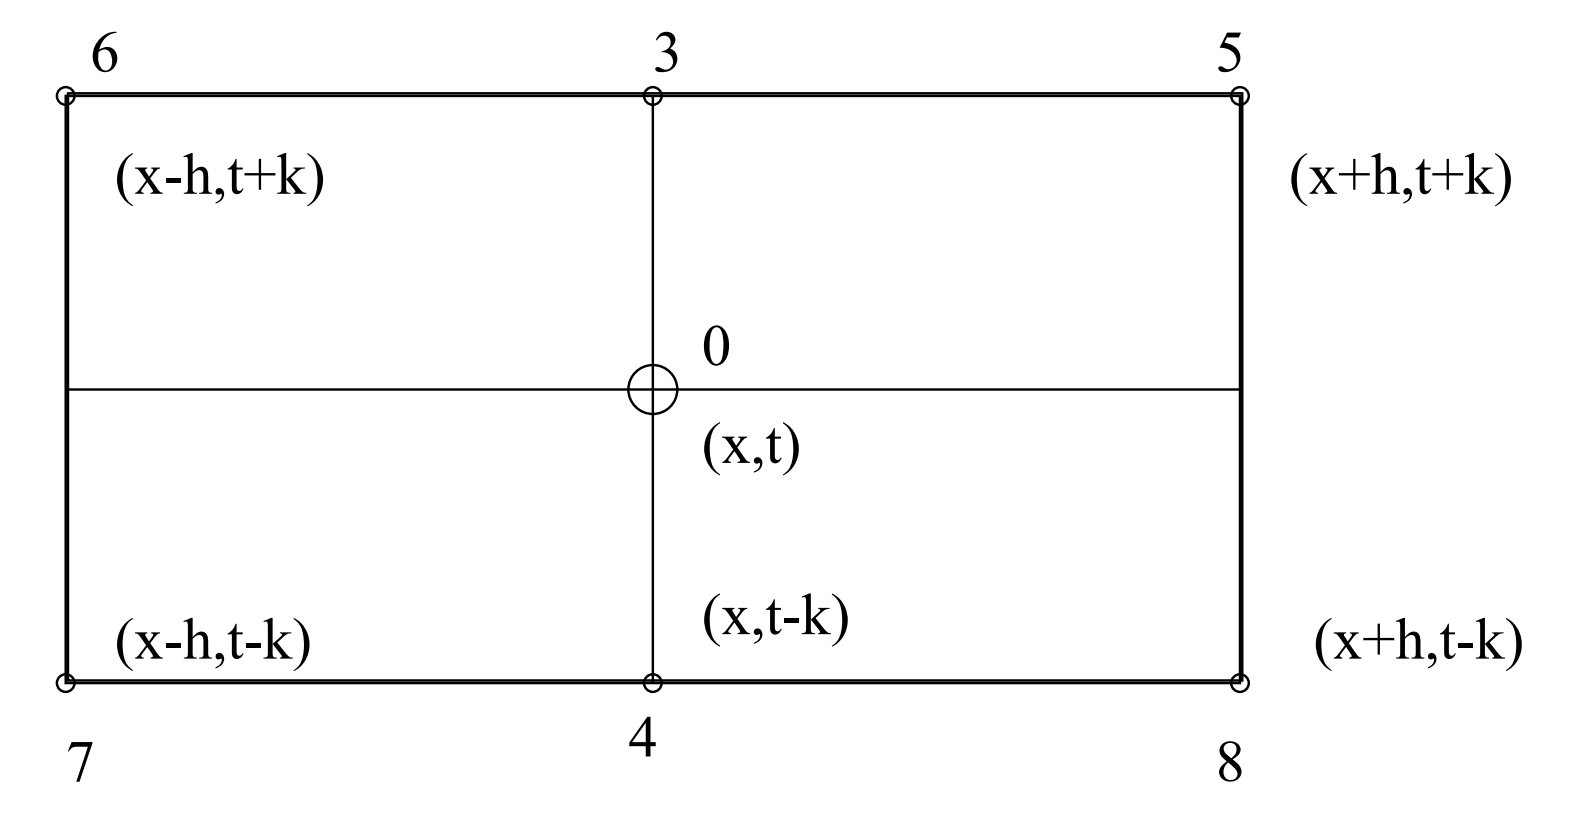
\includegraphics[height = 0.62 \textheight]{img/23/implicit_for_initial}}
\end{frame}


\begin{frame}
\begin{multline}U_{xx}(x,t) = \frac{1}{2} \left [ \frac{u(x-h,t+k) -2u(x,t+k)+u(x+h,t+k)}{h^2} \right. \\
 \left.+ \frac{u(x-h,t-k)-2u(x,t-k)+u(x+h,t-k)}{h^2}\right ]\end{multline}
\vspace{2mm}
\begin{equation}u_{tt}(x,t) =  \frac{u(x,t+k)-2u(x,t)+u(x,t-k)}{k^2} \end{equation}
\vspace{2mm}
\begin{equation}u_6 -2 \left (1 + \frac{h^2}{k^2} \right )u_2 + u_5 = -u_7 +2\left (1 + \frac{h^2}{k^2}\right ) u_4 - u_8 - 4 \frac{h^4}{k^4}u_0\end{equation}
\vspace{2mm}
\center{$\rightarrow$ układ równań z macierzą trójdiagonalną}
\end{frame}


\subsection{Mildy Nonlinear Problems}
\begin{frame}{Mildy Nonlinear Problems}
\begin{block}{}
\begin{equation}u_{xx} - u_{tt} = f(x,t,u) \end{equation}
\end{block}
W metodzie jawnej: \\

\begin{equation} \begin{split} \frac{u(x-h,t) - 2 u(x,t) + u(x_h,t)}{h^2} - \frac{u(x,t+k) - 2u(x,t) + u(x,t-k)}{k^2} \\
= f(x,t,u(x,t)) \end{split} \end{equation}
\end{frame}

\begin{frame}
\textbf{The Cauchy Problem -- D'Alambert formula}
 \centerline{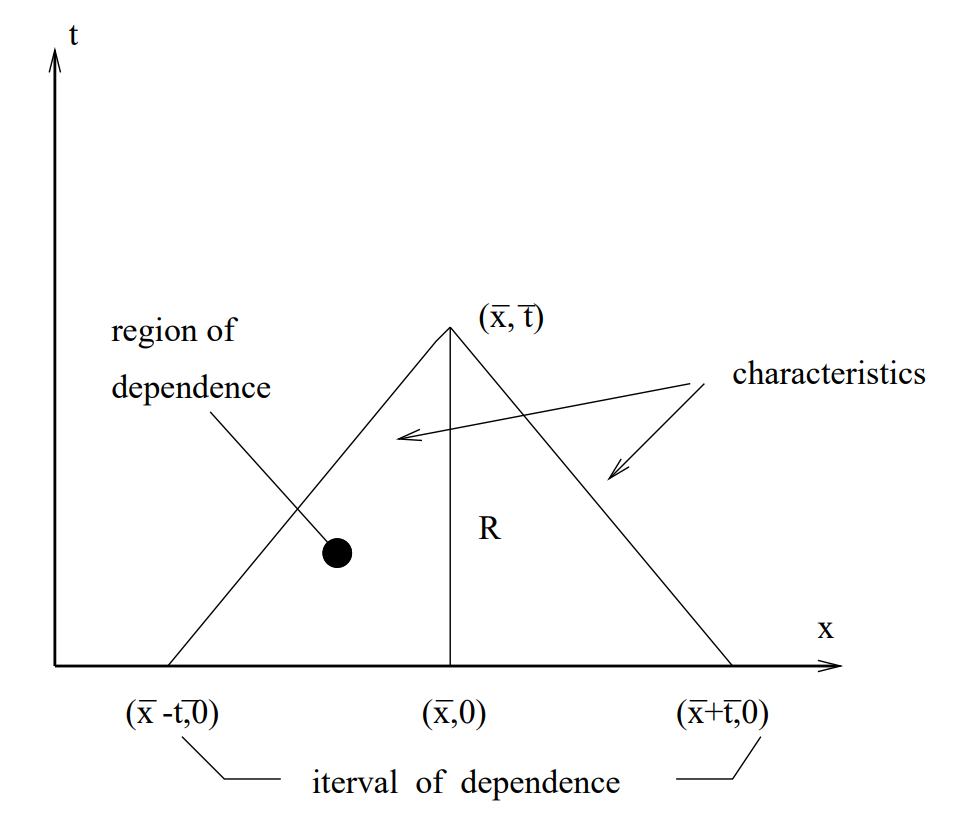
\includegraphics[height = 0.8 \textheight]{img/23/mildy_nonlinear}}
\vspace{5mm}

\end{frame}

\begin{frame}
\begin{equation}u(\overrightarrow{x},\overrightarrow{t}) = \frac{1}{2}\cdot \left [f_1(\overrightarrow{x}+\overrightarrow{t}+f - 1(\overrightarrow{x} -\overrightarrow{t}) +\int_{\overrightarrow{x}-\overrightarrow{t}}^{\overrightarrow{x}+\overrightarrow{t}} f_2(r)dr
\right ] \end{equation}
$u(\overrightarrow{x},\overrightarrow{t})$ jest w sposób kompletny określone przez $f_1, f_2$ \\
dla $x \in [(\overrightarrow{x}-\overrightarrow{t},0),(\overrightarrow{x}+\overrightarrow{t},0)]$

charakterystyki:
\begin{equation} t - \overrightarrow{t} = x - \overrightarrow{x}   \quad t - \overrightarrow{t} = -x - \overrightarrow{x}\end{equation}
\vspace{1mm}
Gdy warunek początkowy zadany dla $0 \le x \le a$ wtedy rozwiązanie tylko dla obszaru zależności
 \centerline{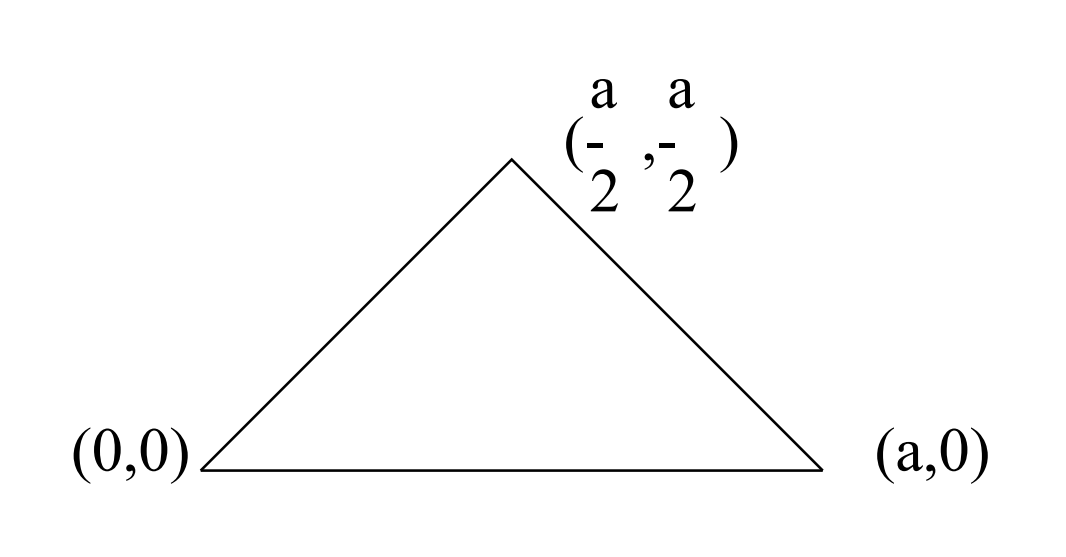
\includegraphics[height = 0.4 \textheight]{img/23/mildy_nonlinear2}}
\end{frame}




 \section{Bibliografia}

  \begin{frame}{Bibliografia}
      \begin{thebibliography}{9}
          \setbeamertemplate{bibliography item}[online]
      				\bibitem{dos}{Mathematics Archives \newblock  Windows/MSDos Software Collection for PDE \newblock \url{http://archives.math.utk.edu/software/msdos/partial.diff.equations/}}
      \end{thebibliography}
  \end{frame}

\end{document}
